\documentclass[tikz,border=12pt]{standalone}
\usepackage[T1]{fontenc}
\usepackage{mathpazo}
\usepackage{amsmath,amssymb}
\usetikzlibrary{arrows.meta, positioning, calc, backgrounds, fit}

\definecolor{stblue}{HTML}{7B97AD}
\definecolor{rwgold}{HTML}{B8995E}
\definecolor{sage}{HTML}{7A9A7E}
\definecolor{dkbrown}{HTML}{3D3530}
\definecolor{wmgray}{HTML}{7B7067}
\definecolor{cream}{HTML}{F9F6F0}
\definecolor{border}{HTML}{D4C9B8}
\definecolor{terracotta}{HTML}{C47A6A}
\definecolor{lavender}{HTML}{907EA0}
\definecolor{copper}{HTML}{A58B6D}

\begin{document}
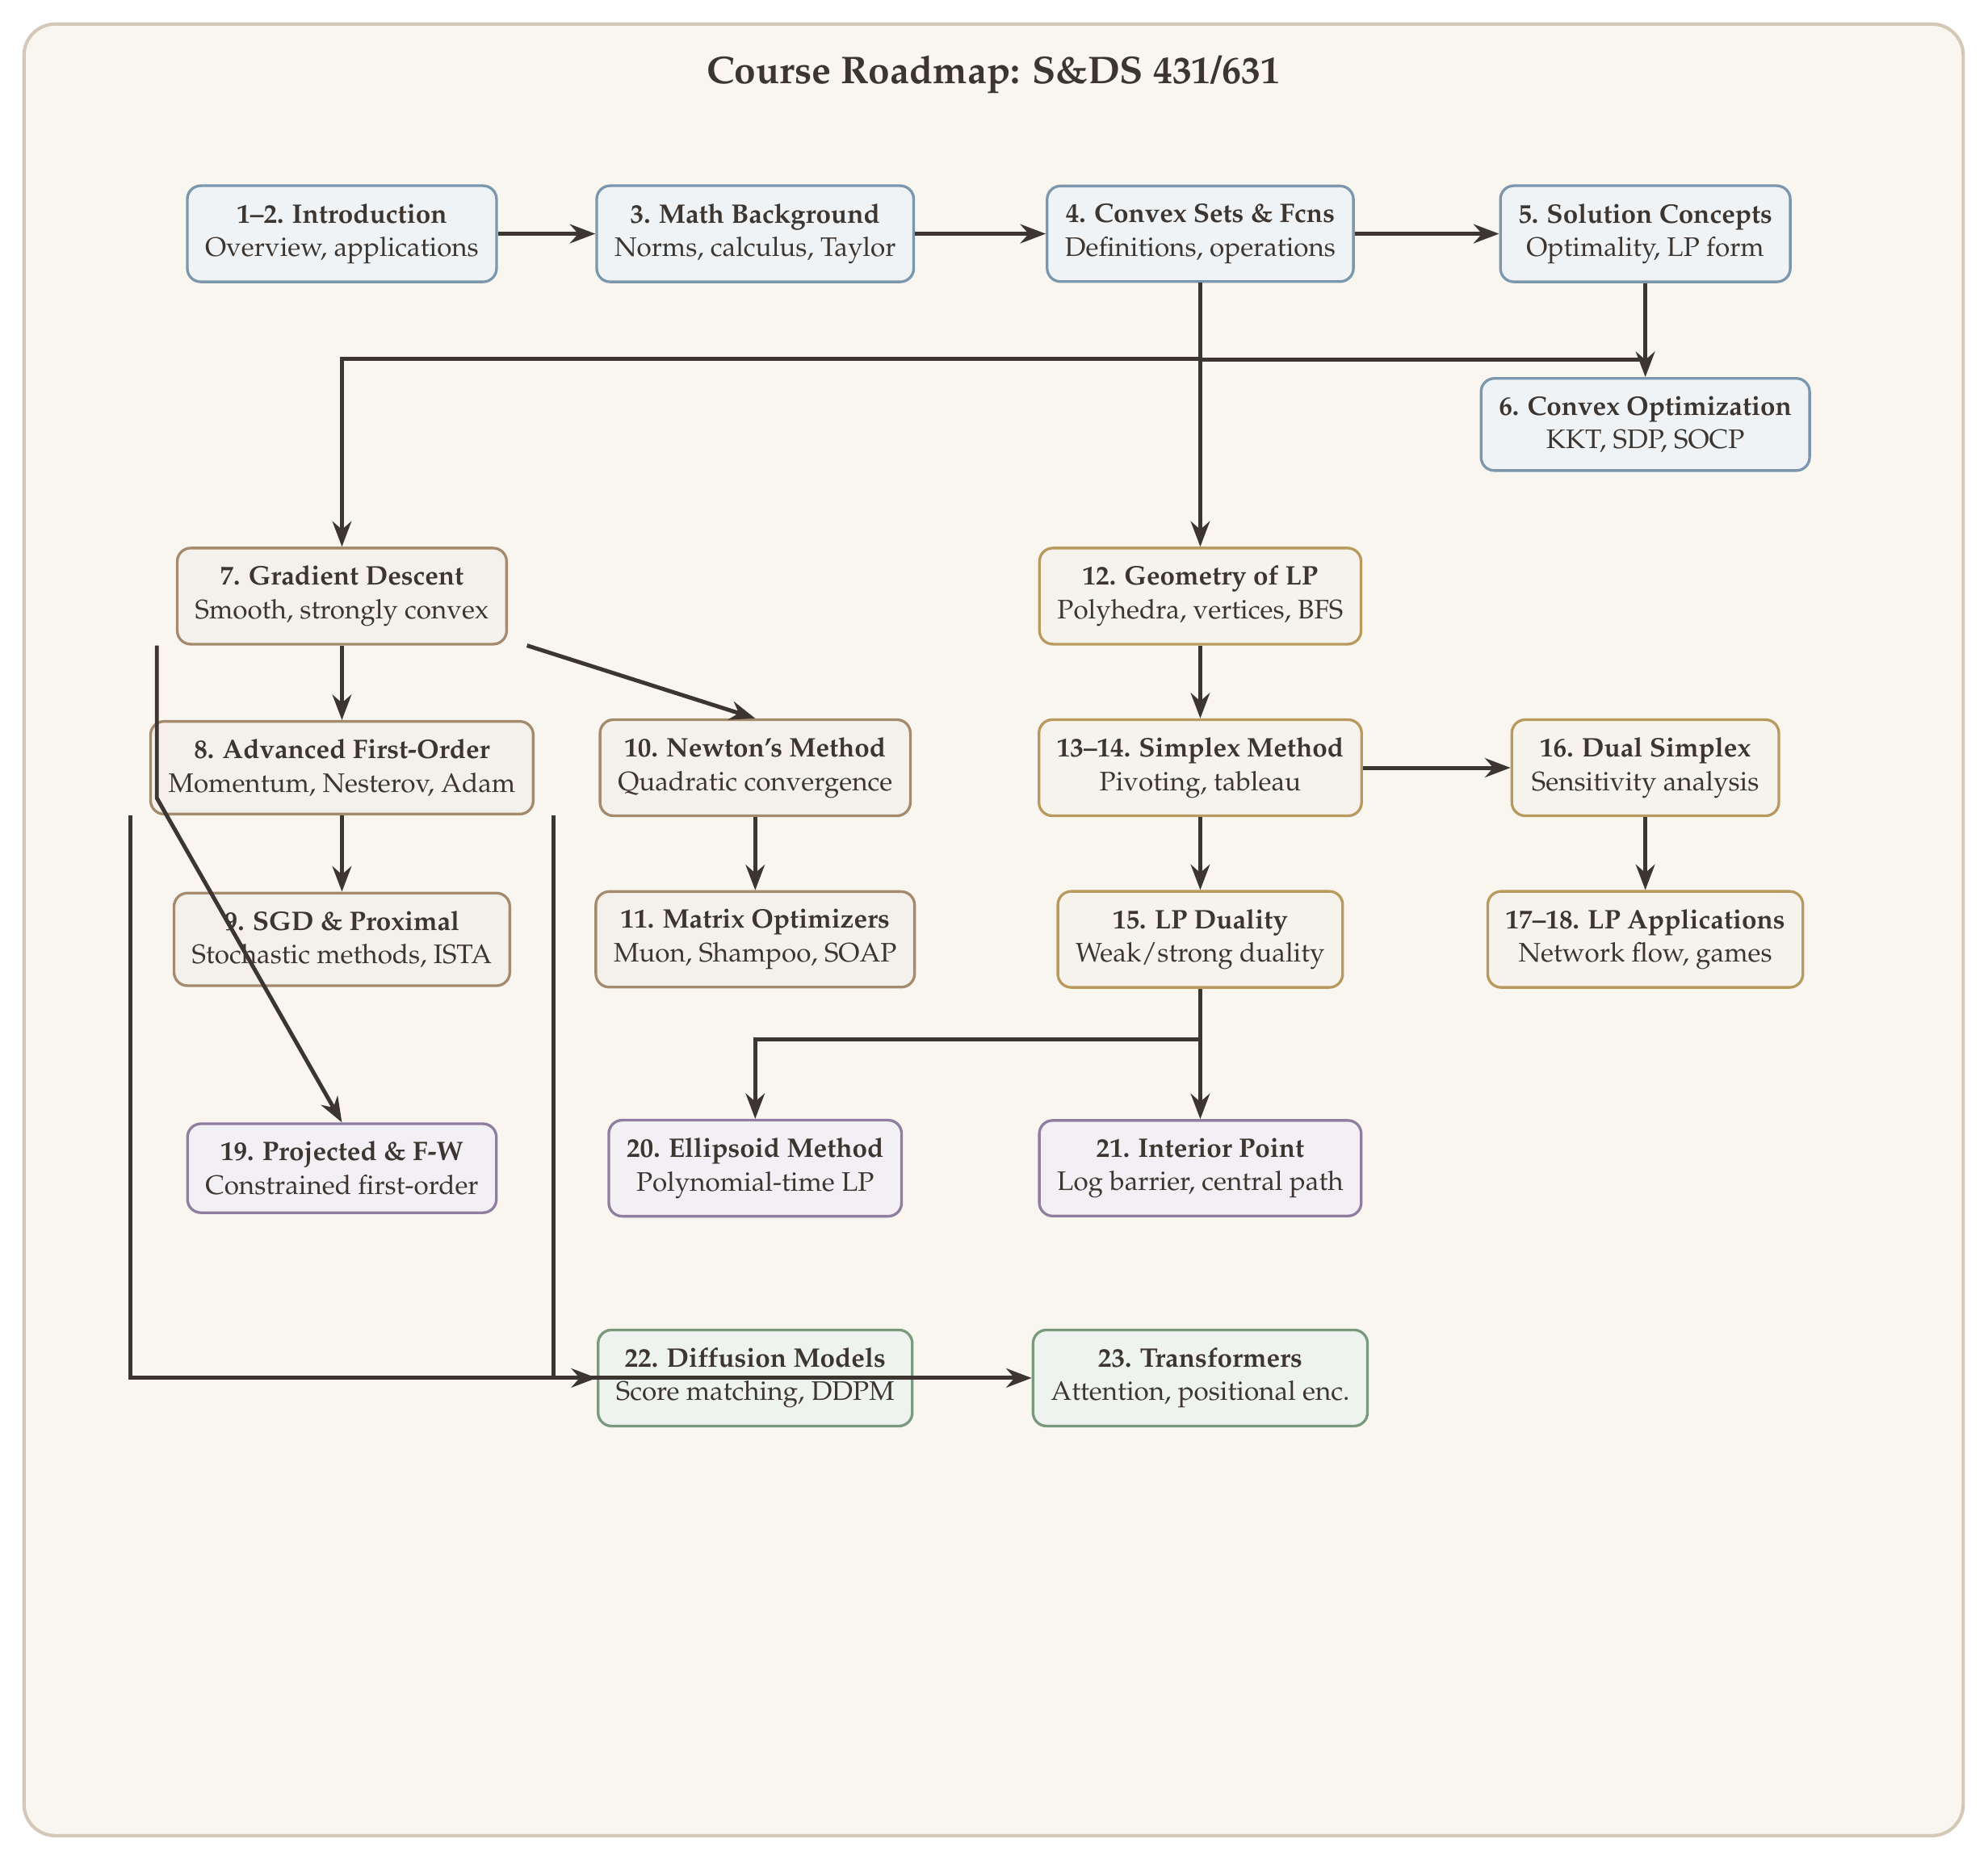
\begin{tikzpicture}[
  >={Stealth[length=4mm, width=3mm]},
  chbox/.style={rounded corners=6pt, line width=1.2pt, minimum height=1.3cm,
                minimum width=4.2cm, text=dkbrown, align=center, inner sep=8pt,
                font=\large},
  partlabel/.style={font=\large\bfseries},
]

% Background
\fill[cream, rounded corners=14pt] (-0.5,-27) rectangle (30,1.5);
\draw[border, line width=1.5pt, rounded corners=14pt] (-0.5,-27) rectangle (30,1.5);

% Title
\node[font=\LARGE\bfseries, text=dkbrown] at (14.75,0.7) {Course Roadmap: S\&DS 431/631};

% =====================================================
% Part I: Foundations (stblue) — Row 0-1
% =====================================================
\node[chbox, fill=stblue!12, draw=stblue] (ch1) at (4.5,-1.8)
  {{\large\bfseries 1--2. Introduction}\\[1pt]{Overview, applications}};

\node[chbox, fill=stblue!12, draw=stblue] (ch3) at (11,-1.8)
  {{\large\bfseries 3. Math Background}\\[1pt]{Norms, calculus, Taylor}};

\node[chbox, fill=stblue!12, draw=stblue] (ch4) at (18,-1.8)
  {{\large\bfseries 4. Convex Sets \& Fcns}\\[1pt]{Definitions, operations}};

\node[chbox, fill=stblue!12, draw=stblue] (ch5) at (25,-1.8)
  {{\large\bfseries 5. Solution Concepts}\\[1pt]{Optimality, LP form}};

\node[chbox, fill=stblue!12, draw=stblue] (ch6) at (25,-4.8)
  {{\large\bfseries 6. Convex Optimization}\\[1pt]{KKT, SDP, SOCP}};

\draw[->, line width=1.8pt, dkbrown] (ch1.east) -- (ch3.west);
\draw[->, line width=1.8pt, dkbrown] (ch3.east) -- (ch4.west);
\draw[->, line width=1.8pt, dkbrown] (ch4.east) -- (ch5.west);
\draw[->, line width=1.8pt, dkbrown] (ch5.south) -- (ch6.north);

% =====================================================
% Part II: First- & Second-Order (copper) — Column left
% =====================================================
\node[chbox, fill=copper!12, draw=copper] (ch7) at (4.5,-7.5)
  {{\large\bfseries 7. Gradient Descent}\\[1pt]{Smooth, strongly convex}};

\node[chbox, fill=copper!12, draw=copper] (ch8) at (4.5,-10.2)
  {{\large\bfseries 8. Advanced First-Order}\\[1pt]{Momentum, Nesterov, Adam}};

\node[chbox, fill=copper!12, draw=copper] (ch9) at (4.5,-12.9)
  {{\large\bfseries 9. SGD \& Proximal}\\[1pt]{Stochastic methods, ISTA}};

\node[chbox, fill=copper!12, draw=copper] (ch10) at (11,-10.2)
  {{\large\bfseries 10. Newton's Method}\\[1pt]{Quadratic convergence}};

\node[chbox, fill=copper!12, draw=copper] (ch11) at (11,-12.9)
  {{\large\bfseries 11. Matrix Optimizers}\\[1pt]{Muon, Shampoo, SOAP}};

\draw[->, line width=1.8pt, dkbrown] (ch4.south) -- ++(0,-1.2) -| (ch7.north);
\draw[->, line width=1.8pt, dkbrown] (ch7.south) -- (ch8.north);
\draw[->, line width=1.8pt, dkbrown] (ch8.south) -- (ch9.north);
\draw[->, line width=1.8pt, dkbrown] (ch7.south east) ++(0.3,0) -- (ch10.north);
\draw[->, line width=1.8pt, dkbrown] (ch10.south) -- (ch11.north);

% =====================================================
% Part III: Linear Programming (rwgold) — Column center-right
% =====================================================
\node[chbox, fill=rwgold!12, draw=rwgold] (ch12) at (18,-7.5)
  {{\large\bfseries 12. Geometry of LP}\\[1pt]{Polyhedra, vertices, BFS}};

\node[chbox, fill=rwgold!12, draw=rwgold] (ch13) at (18,-10.2)
  {{\large\bfseries 13--14. Simplex Method}\\[1pt]{Pivoting, tableau}};

\node[chbox, fill=rwgold!12, draw=rwgold] (ch14) at (18,-12.9)
  {{\large\bfseries 15. LP Duality}\\[1pt]{Weak/strong duality}};

\node[chbox, fill=rwgold!12, draw=rwgold] (ch15) at (25,-10.2)
  {{\large\bfseries 16. Dual Simplex}\\[1pt]{Sensitivity analysis}};

\node[chbox, fill=rwgold!12, draw=rwgold] (ch16) at (25,-12.9)
  {{\large\bfseries 17--18. LP Applications}\\[1pt]{Network flow, games}};

\draw[->, line width=1.8pt, dkbrown] (ch5.south) -- ++(0,-1.2) -| (ch12.north);
\draw[->, line width=1.8pt, dkbrown] (ch12.south) -- (ch13.north);
\draw[->, line width=1.8pt, dkbrown] (ch13.south) -- (ch14.north);
\draw[->, line width=1.8pt, dkbrown] (ch13.east) -- (ch15.west);
\draw[->, line width=1.8pt, dkbrown] (ch15.south) -- (ch16.north);

% =====================================================
% Part IV: Constrained (lavender) — Row bottom-left
% =====================================================
\node[chbox, fill=lavender!12, draw=lavender] (ch17) at (4.5,-16.5)
  {{\large\bfseries 19. Projected \& F-W}\\[1pt]{Constrained first-order}};

\node[chbox, fill=lavender!12, draw=lavender] (ch18) at (11,-16.5)
  {{\large\bfseries 20. Ellipsoid Method}\\[1pt]{Polynomial-time LP}};

\node[chbox, fill=lavender!12, draw=lavender] (ch19) at (18,-16.5)
  {{\large\bfseries 21. Interior Point}\\[1pt]{Log barrier, central path}};

\draw[->, line width=1.8pt, dkbrown] (ch7.south west) ++(-0.3,0) -- ++(0,-2.4) -- (ch17.north);
\draw[->, line width=1.8pt, dkbrown] (ch14.south) -- ++(0,-0.8) -| (ch18.north);
\draw[->, line width=1.8pt, dkbrown] (ch14.south) -- ++(0,-0.8) -| (ch19.north);

% =====================================================
% Part V: Advanced Topics (sage) — Row bottom
% =====================================================
\node[chbox, fill=sage!12, draw=sage] (ch20) at (11,-19.8)
  {{\large\bfseries 22. Diffusion Models}\\[1pt]{Score matching, DDPM}};

\node[chbox, fill=sage!12, draw=sage] (ch21) at (18,-19.8)
  {{\large\bfseries 23. Transformers}\\[1pt]{Attention, positional enc.}};

\draw[->, line width=1.8pt, dkbrown] (ch8.south west) ++(-0.3,0) |- (ch20.west);
\draw[->, line width=1.8pt, dkbrown] (ch8.south east) ++(0.3,0) |- (ch21.west);

% =====================================================
% Part region shading
% =====================================================
\begin{pgfonlayer}{background}
  % Part I: Foundations
  \fill[stblue!5, rounded corners=10pt] (1.5,-0.6) rectangle (28.5,-5.8);
  \node[partlabel, text=stblue!60] at (2.8,-0.9) {Part I: Foundations};

  % Part II: First- and Second-Order
  \fill[copper!5, rounded corners=10pt] (1.5,-6.3) rectangle (14.2,-14);
  \node[partlabel, text=copper!60] at (2.8,-6.6) {Part II: Optimization};

  % Part III: Linear Programming
  \fill[rwgold!5, rounded corners=10pt] (14.8,-6.3) rectangle (28.5,-14);
  \node[partlabel, text=rwgold!60] at (16.3,-6.6) {Part III: Linear Programming};

  % Part IV: Constrained
  \fill[lavender!5, rounded corners=10pt] (1.5,-15.2) rectangle (21.2,-17.8);
  \node[partlabel, text=lavender!60] at (2.8,-15.5) {Part IV: Constrained};

  % Part V: Advanced
  \fill[sage!5, rounded corners=10pt] (7.8,-18.5) rectangle (21.2,-21.1);
  \node[partlabel, text=sage!60] at (9.1,-18.8) {Part V: Advanced Topics};
\end{pgfonlayer}

\end{tikzpicture}
\end{document}
